% !Tex TS-program = lualatex
\documentclass[a4paper,10pt]{article}
\usepackage[utf8]{inputenc}
\usepackage{src/preamble}
\usepackage[
	backend=biber,
	maxalphanames=10,
]{biblatex}
\bibliography{bibliography.bib}

\begin{document}

\noindent
\begin{center}
	\textbf{{EFFICIENT SOLUTION FOR MST COMPUTATION ON SPARSE GRAPHS}} \\
\end{center}

\noindent
\textbf{Author: Alessandro Biagiotti} \hfill \textit{Milan university}
\\

\noindent
\textbf{ABSTRACT:}
\\
In this report I will be explaining the development process for my solution of the widely known \mstp. In the following I will be covering: the problem on a theoretical level~\ref{sec:intro}, the structure I chose to implement to keep the Graph structure in memory~\ref{sec:graph-structure}, briefly the CPU implementation~\ref{sec:cpu-implementation} and my GPU implementation~\ref{sec:gpu-implementation}, the results in terms of speedup and occupancy~\ref{sec:performance-analysis} and finally some conclusions regarding the project and the problem as a whole~\ref{sec:final-thoughts}.

\bigskip

\phantomsection
\makeatletter\def\@currentlabel{\texttt{(I)}}\makeatother\label{sec:intro}
\noindent
\textbf{INTRODUCTION TO THE PROBLEM:}
\\
The Minimum Spanning Tree Problem (\mstp for short) is a problem that has been studied for years and to this day finds many real world applications,to name a few:
\begin{enumerate}
	\item It's possible to find different \mst-based techniques used to do image segmentation~\cite{maze-generation}~\cite{mst-segmentation-heuristic}.
	\item Finding an \mst allows us to solve the Clustering problem, all we need to do is to compute an \mst and then drop its $k - 1$ most expensive edges~\cite{mst-applications}.
	\item Finding an \mst is an important step of Christofides's algorithm, which is a 2-approximation for the widely known Travelling Salesman Problem (\textsc{Tsp} for short)~\cite{tsp-christofides}.
\end{enumerate}

Many different solutions have been found for the problem in the years, the more basic implementations were Prim's~\cite{prim-algorithm} and Kruskal's~\cite{kruskal-algorithm}.

Prim's algorithm is the simplest solver for \mstp, given a graph $G= (V, E)$, let us suppose that the size of the graph $|V|$ is $n$ and the number of edges $|E|$ is $m$, then, based on the implementation, the computational complexity varies:
\begin{itemize}
	\item Na\"ive implementation: $\O(n^2)$
	\item Binary heap and adjacency list: $\O(m\log{n})$
	\item Fibonacci heap and adjacency list: $\O(m + n\log{n})$
\end{itemize}
In my implementation I have implemented both the Na\"ive version and the one using a binary heap, more on this in section~\ref{sec:cpu-implementation}.

Kruskal's algorithm is the alternative to Prim's algorithm and it works in time $\O(m\log{m})$ if implemented using classical data structures.

\brka's algorithm is a solver for the \mstp based on forests, a more verbose version of the algorithm shown in~\cite{boruvka-pseudocode} can be found in~\ref{algo:boruvka-pseudocode}
\begin{algorithm}
	\caption{\brka's algorithm}
	\label{algo:boruvka-pseudocode}
	\begin{algorithmic}[1]
		\REQUIRE An undirected, connected and weighted graph $G$, a set of empty edges $T$
		\ENSURE An \mst$T$ built on graph $G$
		\WHILE{vertices in $G$ connected by $T$ are disjoint}
		\STATE start with an empty set of edges $E$
		\FOR{every connected component}
		\STATE start with an empty set of edges $S$
		\FOR{every vertex $v$ in the component}
		\STATE add the cheapest edge going from $v$ to any other component to $S$
		\ENDFOR
		\STATE add the cheapest edge in $S$ to $E$
		\ENDFOR
		\STATE add the set of edges from $E$ to $T$
		\ENDWHILE
		\STATE\RETURN $T$
	\end{algorithmic}
\end{algorithm}

Let us suppose that the size of the graph $|V|$ is $n$ and the number of edges $E$ is $m$, then the computational complexity of the pseudocode shown in~\ref{algo:boruvka-pseudocode} is $\O(m\log{n})$. This algorithm has been later reused in combination with other techniques to compute a solution for the \mstp very efficiently~\cite{boruvka-ackermann}~\cite{karger-klein-tarjan}.

While parallel solutions based on Prim's or Kruskal's algorithm exists like~\cite{prim-parallel}~\cite{filter-kruskal} \brka's solver gained more traction thanks to its inherent parallelizability. Regardless of the implementation the core of the parallel variant can be identified in the following four steps as identified in~\cite{boruvka-steps}:
\begin{enumerate}
	\item\label{item:first-step} (\textit{choose lightest}) for every vertex the lightest edge is chosen in parallel.
	\item\label{item:second-step} (\textit{find root}) for every vertex we find the root of the tree to which it belongs\footnote{It's important to keep in mind that vertices are actually supervertices.}.
	\item\label{item:third-step} (\textit{rename vertices}) Since the graph after~\ref{item:fourth-step} is compressed, which means that the number of vertices decreases, then the roots in the graph need to be renamed.
	\item\label{item:fourth-step} (\textit{graph compression}) The graph undergoes a compression step, the resulting graph will contain only the roots identified during~\ref{item:second-step} and the edges that connect component $\mathcal{C}_i$ to any other component $\mathcal{C}_j$, any edge contained within a component will be lost.
\end{enumerate}

The specific implementation that I chose to follow is shown in~\cite{generic-he-boruvka} and is summarized by algorithm~\ref{algo:boruvka-parallel}

\begin{algorithm}
	\caption{\brka's algorithm}\label{algo:boruvka-parallel}
	\begin{algorithmic}[1]
		\REQUIRE An undirected, connected and weighted graph $G(V, E)$
		\ENSURE An \mst$T$ built on graph $G$
		\WHILE{$|V| > 1$}
		\STATE find the minimum edge per vertex (\ref{item:first-step})
		\STATE remove mirrored edges
		\STATE initialize the colors
		\WHILE{the coloring hasn't converged}
		\STATE color propagation (\ref{item:second-step})
		\ENDWHILE
		\STATE create new vertex ids (\ref{item:third-step})
		\STATE do graph compression (\ref{item:fourth-step})
		\ENDWHILE
		\STATE\RETURN $G$
	\end{algorithmic}
\end{algorithm}

The graph returned in the last step is a single supervertex containing the \mst.

\bigskip
\phantomsection
\makeatletter\def\@currentlabel{\texttt{(II)}}\makeatother\label{sec:graph-structure}
\noindent
\textbf{GRAPH STRUCTURE:}
\\
Before discussing the solution I want to introduce the memorization strategy for the graph structure. When working with graphs in CPU code it's common to choose between to alternatives:
\begin{itemize}
	\item The \emph{adjacency matrix}, which represents any connection between two vertices, $i, j$ in the graph as a $1$ or a $0$ in a matrix\footnote{For simplicity's sale I consider an unweighted graph}. Let's suppose that the $|V|$ is $n$, then the amount of space occupied by a matrix in memory is $\O(n^2)$ while the cost of accessing element $(i, j)$, independently from the values of $i$ and $j$, is just $\O(1)$.
	\item The \emph{adjacency list}, which stores only a reference to the neighbour for every node, usually memorized as an array of lists, therefore if $j$ is neighbour for vertex $i$ a reference to $j$ will be placed in the list of neighbours of $i$. Supposing that $|E|$ is $m$, then the cost of keeping such a structure in memory is $O(m + n)$.
\end{itemize}
The approach I followed for the implementation of the algorithm is, to quote the authors of~\cite{generic-he-boruvka} "a compromise between adjacency list and adjacency matrix". The \csr format is a form of encoding linearizing the structure of adjacency lists, to save space, using arrays to keep the adjacency lists in memory, to save time on the accesses. The number of additional arrays implemented in \csr vary slightly in the literature~\cite{csr-kelly}~\cite{csr-wheatman}~\cite{generic-he-boruvka}, for my implementation I chose to stray from the 4-vector solution since it would have only complicated the structure of the graph without holding any additional information:
\begin{itemize}
	\item A \emph{cumulated degrees} array, it's an array cumulating the degrees of the vertices in the graph.
	\item An \emph{neighbours} array, which is a linearization of the graph's adjacency list.
	\item A \emph{weights} array, containing the weight of every edge $(i, j)$ in the graph.
\end{itemize}

\bigskip
\phantomsection
\makeatletter\def\@currentlabel{\texttt{(III)}}\makeatother\label{sec:cpu-implementation}
\noindent
\textbf{CPU IMPLEMENTATION:}
\\
I will not cover at length the CPU implementation since it's quite straightforward, at first I opted
for an extremely na\"ive implementation of Prim's algorithm, consisting of two \texttt{for} cycles.
Since the implementation worked but was in fact extremely slow if compared to finer solvers I
decided to scrap it in favour of a more efficient implementation of the Prim's algorithm based on
the use of a simple heap to sort the edges needed to build the \mst.

Since the time complexity of Prim's solver thus implemented is $\O(m \cdot \log{n})$, as shown in\ref{sec:intro}. I decided to implement Prim's algorithm instead of \brka's solver since the first one is much simpler and, as far as efficiency goes, the two solvers have comparable speeds.

\bigskip
\phantomsection
\makeatletter\def\@currentlabel{\texttt{(IV)}}\makeatother\label{sec:gpu-implementation}
\noindent
\textbf{GPU IMPLEMENTATION:}
\\
As I alluded to in~\ref{sec:intro} I chose to follow~\cite{generic-he-boruvka} as my primary source. In the paper the researchers propose an higlhly efficient and parallel variant of \brka's solver for the GPU.

Per~\cite{generic-he-boruvka} every part of the solution can be implemented as a distinct kernel
deploying a thread per vertex (such an approach is referred to as \textit{topologic} in the
literature)
\begin{enumerate}
	\item\label{item:choose-lightest} (\textit{choose lightest}) this operation picks the
	lightest connection for every vertex to the neighbourhood by simpling cycling over
	the outgoing edges, to have improved locality if two edges share the same weight pick the one with the smaller destination id. The results are stored in the \texttt{d\_candidates} array.
	\item\label{item:mirror-removal} (\textit{Remove mirrored edges}) this operation is meant to
	remove cycles from the graph. To understand how it works let's suppose for a moment
	that the candidate edge for vertex $v$ is $(v, u)$, let's now suppose that the
	candidate edge for $u$ is the mirrored edge $(u, v)$, then the kernel will replace
	$(v, u)$ contained in \texttt{d\_candidates} with the default value
	\texttt{UINT\_MAX}.
	\item\label{item:coloration} (\textit{Initialize and propagate the colors}) this operation
	is meant to identify the connected components inside the graph and can be
	implemented as a recursive procedure having a kernel as the recursion head and then
	a series of \texttt{\_\_device\_\_} function calls to propagate the colors in the nodes\footnote{This operation can probably be implemented with Dynamic Parallelism and a series of \textit{Fire and forget kernels} alongside a \textit{Tail launch} kernel to recover the necessary data}.
	\item\label{item:vertex-rename} (\textit{Create new vertex ids}) to rename the vertices a
	new array is created (in my implementation is \texttt{d\_flag}) that contains a $0$
	in every position where the color of the vertex is different from the vertex id and
	a $1$ otherwise.

	%% NNHCPT
	To understand why the re-labelling is necessary we can consider for instance a graph
	in which we only have $2$ colors but one of the colored vertices is $0$ and the
	other one is $750$, if the vertex id did not change some other technique would need
	to be invented to solve the next step.
	%%
	\item\label{item:graph-contraction} (\textit{Count, assign and insert new edges}) this
	operation needs to be split in a series of simpler kernels
	\begin{itemize}
		\item\label{item:count-edges} (\textit{Count edges}) A simple kernel will be
		going through the neighbourhood of every vertex and it compares the
		color of the vertex with the color of the supervertex of the
		destination. If the colors are different it means that the two
		supervertices belong to different components.

		The result of the process will be cumulated inside an array (in my
		implementation is \texttt{d\_cumDegs})

		Afterwards a scan procedure is computed on the \texttt{d\_cumDegs}
		array, the result is going to be a fully functioning cumulated
		degree array as shown in~\ref{sec:graph-structure}.
		\item\label{item:graph-regen} (\textit{Graph regeneration}) This step
		generates the new neighbour and weight array, this is done by
		visiting every neighbour for every vertex as shown in~\ref{item:count-edges}. Edges intra-component are removed while duplicated ones are kept because it's easier than handling their removal.
	\end{itemize}
\end{enumerate}
Most of the kernels proposed in the solution can be written as \texttt{for} loops that go through
the various neighbours in the adjacency lists and, since there is no dependency between the various vertices~\cite{generic-he-boruvka}, the various steps can be computed in parallel for a major efficiency boost. Synchronization is only ever needed inside the \texttt{scan} functions, to make sure that all of the threads have a consistent view of shared memory, furthermore atomic operations are required in some instances to offer a solution to race conditions.

\bigskip
\phantomsection
\makeatletter\def\@currentlabel{\texttt{(III)}}\makeatother\label{sec:performance-analysis}
\noindent
\textbf{PERFORMANCE ANALYSIS:}
\\
Performance analysis has been carried out using an online machine through the Google Colab hosting service\footnote{\url{https://colab.research.google.com/}}, the machine specs, gathered through tools like \texttt{/proc/cpuinfo} and \texttt{/proc/meminfo}, alongside \texttt{nvidia-smi} and the official documentation~\cite{t4-info}~\cite{t4-product-brief}, are listed in~\ref{tbl:system}
\begin{center}
	\begin{longtable}{|c|c|c|}
		\caption{System information}\label{tbl:system}
		\\\hline\textbf{} & \textbf{CPU} & \textbf{GPU} \\\hline\hline
		\endfirsthead\hline\endlastfoot

		\textbf{Manufacturer}               & Intel                                                                                                               & NVIDIA                                                              \\\hline

		\textbf{Model}                      & Intel Xeon (V\footnote{V stands for virtualized, can't find the actual CPU model that is being mounted in servers}) & T4                                                                  \\\hline
		\textbf{Launch Date}                & N.A.                                                                                                                & Oct 2018                                                            \\\hline
		\textbf{\#Cores}                    & $2$ vcores                                                                                                          & $\num{2560}$ C\footnote{CUDA cores}, $320$ T\footnote{Tensor cores} \\\hline
		\textbf{Clock Speed (GHz)}          & $\num{2.20}$ GHz                                                                                                    & Base: $0.585$ MHz, Boost: $1.59$ GHz                                \\\hline
		\textbf{Memory / Cache}             & L3 Cache: $56$ MB                                                                                                   & VRAM: $16$ GB GDDR6                                                 \\\hline
		\textbf{Memory Bandwidth}           & N.A.                                                                                                                & 300 GB/s                                                            \\\hline
		\textbf{TDP (Thermal Design Power)} & N.A.                                                                                                                & $70$ W                                                              \\\hline
		\textbf{Architecture}               & N.A.                                                                                                                & Turing
	\end{longtable}
\end{center}
All of the benchmarks conducted are part of the tests provided for the 9th challenge by DIMACS\footnote{DIscrete MAthematics \& theoretical Computer Science center (\url{https://www.diag.uniroma1.it/challenge9/download.shtml})} center, the tests I used to get the results shown in~\ref{fig:results} are listed in table~\ref{tbl:benchmarks}.
\begin{longtable}{|c|c|c|}
	\caption{Benchmark dimensions}\label{tbl:benchmarks}
	\\\hline\textbf{Benchmark} & \textbf{Node size} & \textbf{Edge size} \\\hline\hline
	\endfirsthead\hline\endlastfoot

	\textit{New York}                & $\num{264346}$   & $\num{733846}$  \\\hline
	\textit{San Francisco, bay area} & $\num{321270}$   & $\num{800172}$  \\\hline
	\textit{Colorado}                & $\num{435666}$   & $\num{1057066}$ \\\hline
	\textit{Florida}                 & $\num{ 070376}$  & $\num{2712798}$ \\\hline
	\textit{California and Nevada}   & $\num{ 1890815}$ & $\num{4657742}$ \\\hline
	\textit{Great Lakes}             & $\num{2758119}$  & $\num{6885658}$ \\\hline
	\textit{Eastern USA}             & $\num{3598623}$  & $\num{8778114}$
\end{longtable}
Before discussing the results I want to point out that my GPU implementation gave very good results compared to the CPU code I wrote in the beginning, therefore in Figure~\ref{fig:results}, I decided to include both the GPU and CPU results listed in the original paper~\cite{generic-he-boruvka}. While I believe the CPU to be directly comparable with my results, since the CPU architecture used to test the code in the source material is closely related to the hardware that is running underneath Colab's environment, the GPU results are there more as a testament to the work that has been done prior.
\begin{figure}
	\centering
	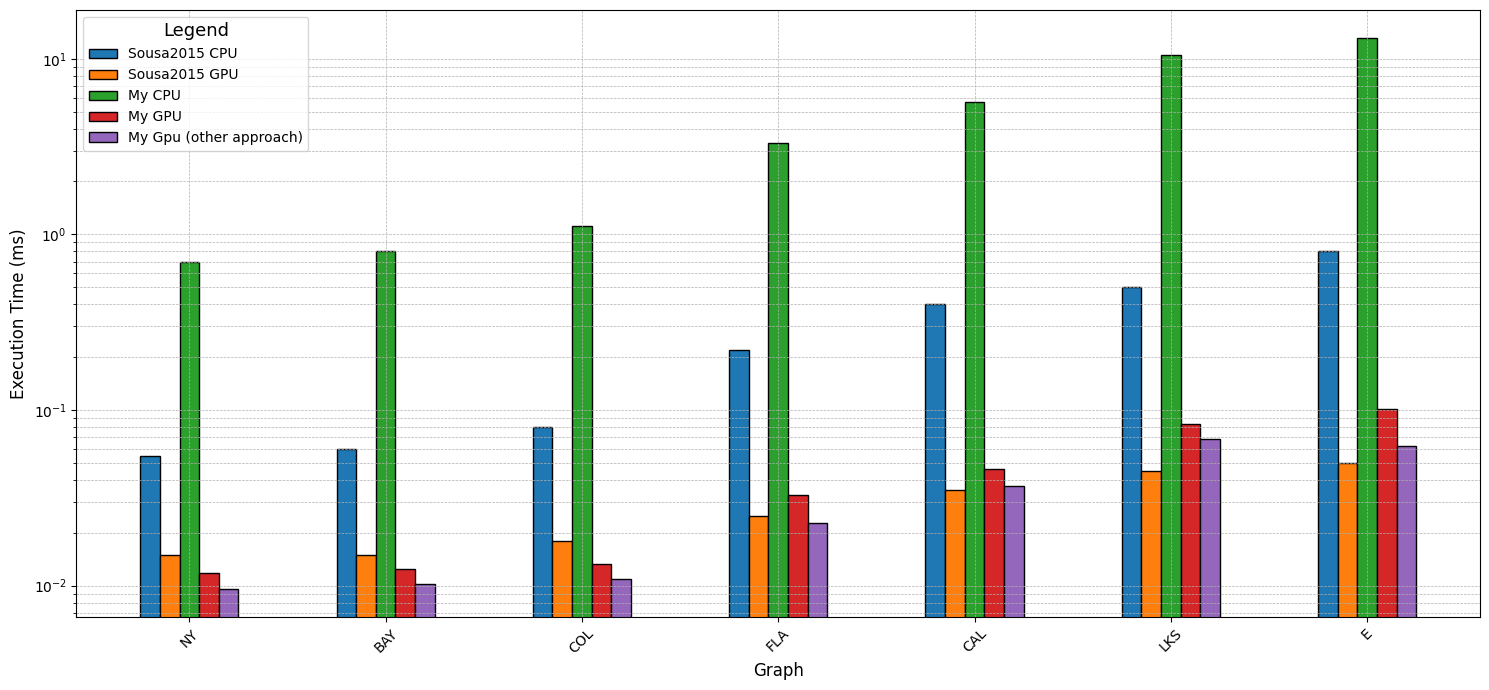
\includegraphics[scale=0.4]{fig/benchmarks.png}
	\caption{Performance metrics for the various platforms compared with the results in \cite{generic-he-boruvka}}
	\label{fig:results}
\end{figure}
Computing the speedups for my GPU code, which is evidently less efficient than the one proposed in~\cite{generic-he-boruvka}, with respect to my CPU the results are in the neighbourhood of $\sim59\times$ to $\sim128\times$. Considering instead the results from the authors I get that the speedup is in between $\sim5\times$ and $\sim8\times$. Doing an analysis of the occupancy of the solution it's clear that it's suffering from the topological approach chosen to solve the problem.

\bigskip
\phantomsection
\makeatletter\def\@currentlabel{\texttt{(IV)}}\makeatother\label{sec:final-thoughts}
\noindent
\textbf{CONCLUSIONS:}
\\
\mstp will never stop to amaze the amount of use that can be made out of the solution of such a simple problem is nothing short of incredible.

In the previous sections I explained how I got to the solution for the problem following somebody else's footsteps but much is still unknown, although the original paper was published under the title "A generic and highly efficient parallel variant of \brka's algorithm" it's immediately clear by taking a look at what kind of tests have been done on the solver (all similar to~\ref{tbl:benchmarks}) it's clear that the solution is far from being "generic" and it's highly likely it will perform as amazing as it does in the benchmarks shown in~\ref{fig:results} only if the graph is actually sparse (or very close to being such).

As soon as the graph becomes more dense the complexity of computing simple kernels like the ones shown in~\ref{sec:gpu-implementation}, which will contain a \texttt{for} loop to comply with the topologic approach, will explode in complexity\footnote{The "critique" I just moved is merely based on speculation because I do not have access to the original source code}.

It would be interesting, in this field, to keep on analyzing further techniques in the field of parallel \mstp solvers, especially in the field of more generic graphs. This can be acheived by analyzing the problem following the same approach I used in this impolementation, therefore solving \mstp through repeated contractions by rank; or by changing completely the way to get to the solution as a group did in~\cite{mst-bipartite} to avoid paying the costs of doing a rank in the graph list, which can be expensive.

\clearpage

\printbibliography

\end{document}
